% ---
% Arquivo com a Introdução do Trabalho de Conclusão de Curso dos alunos
% Gabriel Takaoka Nishimura, Felippe Demarqui Ramos e Vivian Kimie Isuyama 
% da Escola Politécnica da Universidade de São Paulo
% ---
	\chapter*[Introdução]{Introdução} %(exemplo de capítulo sem numeração, mas presente no Sumário)
	\addcontentsline{toc}{chapter}{Introdução}
		
	A saturação das infraestruturas de rádio frequência é iminente \cite{load-balancing}. Apenas no ano de 2015, mais de meio bilhão de telefones celulares foram adicionados à rede de telefonia no mundo \cite{cisco-forecast}. Em relação ao crescimento de aparelhos conectados como carro, geladeiras, TV’s, DVD’s etc, existem previsões de que a sua quantidade chegará a 9 bilhões em 2020, com um crescimento 	de 900\% em relação a 2015 \cite{erricson-report}. O tráfego IP também fica cada vez mais carregado, sendo previsto para atingir 168 exabytes em 2019, como pode-se observar na \autoref{fig_cisco}.
	
	\begin{figure}[!htb]
		\caption{\label{fig_cisco}Gráfico do crescimento do tráfego IP do ano 2014 ao 2019}
		\begin{center}
			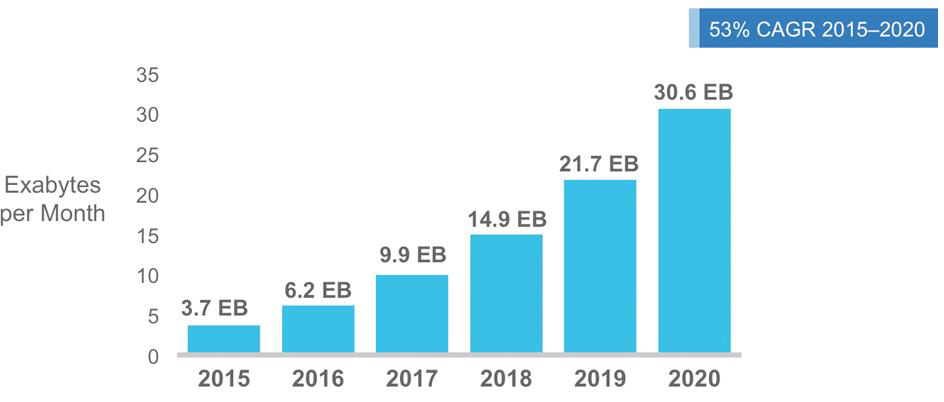
\includegraphics[scale=0.5]{cisco_exabytes_per_month.png}
		\end{center}
		\legend{Fonte: Cisco Visual Networking Index: Global Mobile Data Traffic Forecast Update, p. 5}
	\end{figure}
	
	No Brasil, a Anatel regulamenta uma banda de frequências que pertencem ao intervalo  de 3KHz até 300GHz \cite{faixa-anatel}. Isso significa que existem frequências reservadas para tipos específicos de comunicação, com o intuito de diminuir interferência entre elas. No entanto, essa atribuição deixa aparelhos como telefones sem fio, tablets, roteadores e notebooks em frequências não licenciadas (como 2.4GHz) pois são de livre uso. Eventualmente, o número excessivo de dispositivos conectados em  frequências livres pode causar interferência, com consequências como falha de comunicação generalizada de dispositivos em áreas mais densas. Caso não seja solucionada, a saturação das frequências livres gerará uma crise de conectividade. \par 
	
	Observa-se no entanto, que a luz, cuja frequência pertence ao intervalo de 430THz a 750THz \cite{vision},  não é regulamentada por nenhuma agência (vide \autoref{fig_fcc}), e pode se tornar uma solução para essa crise.

	\begin{figure}[htb]
		\caption{\label{fig_fcc}Caracterização dos espectros de frequências, de 0Hz a 1000THz - frequências reguladas estão em laranja.}
		\begin{center}
		%  trim={<left> <lower> <right> <upper>} 
		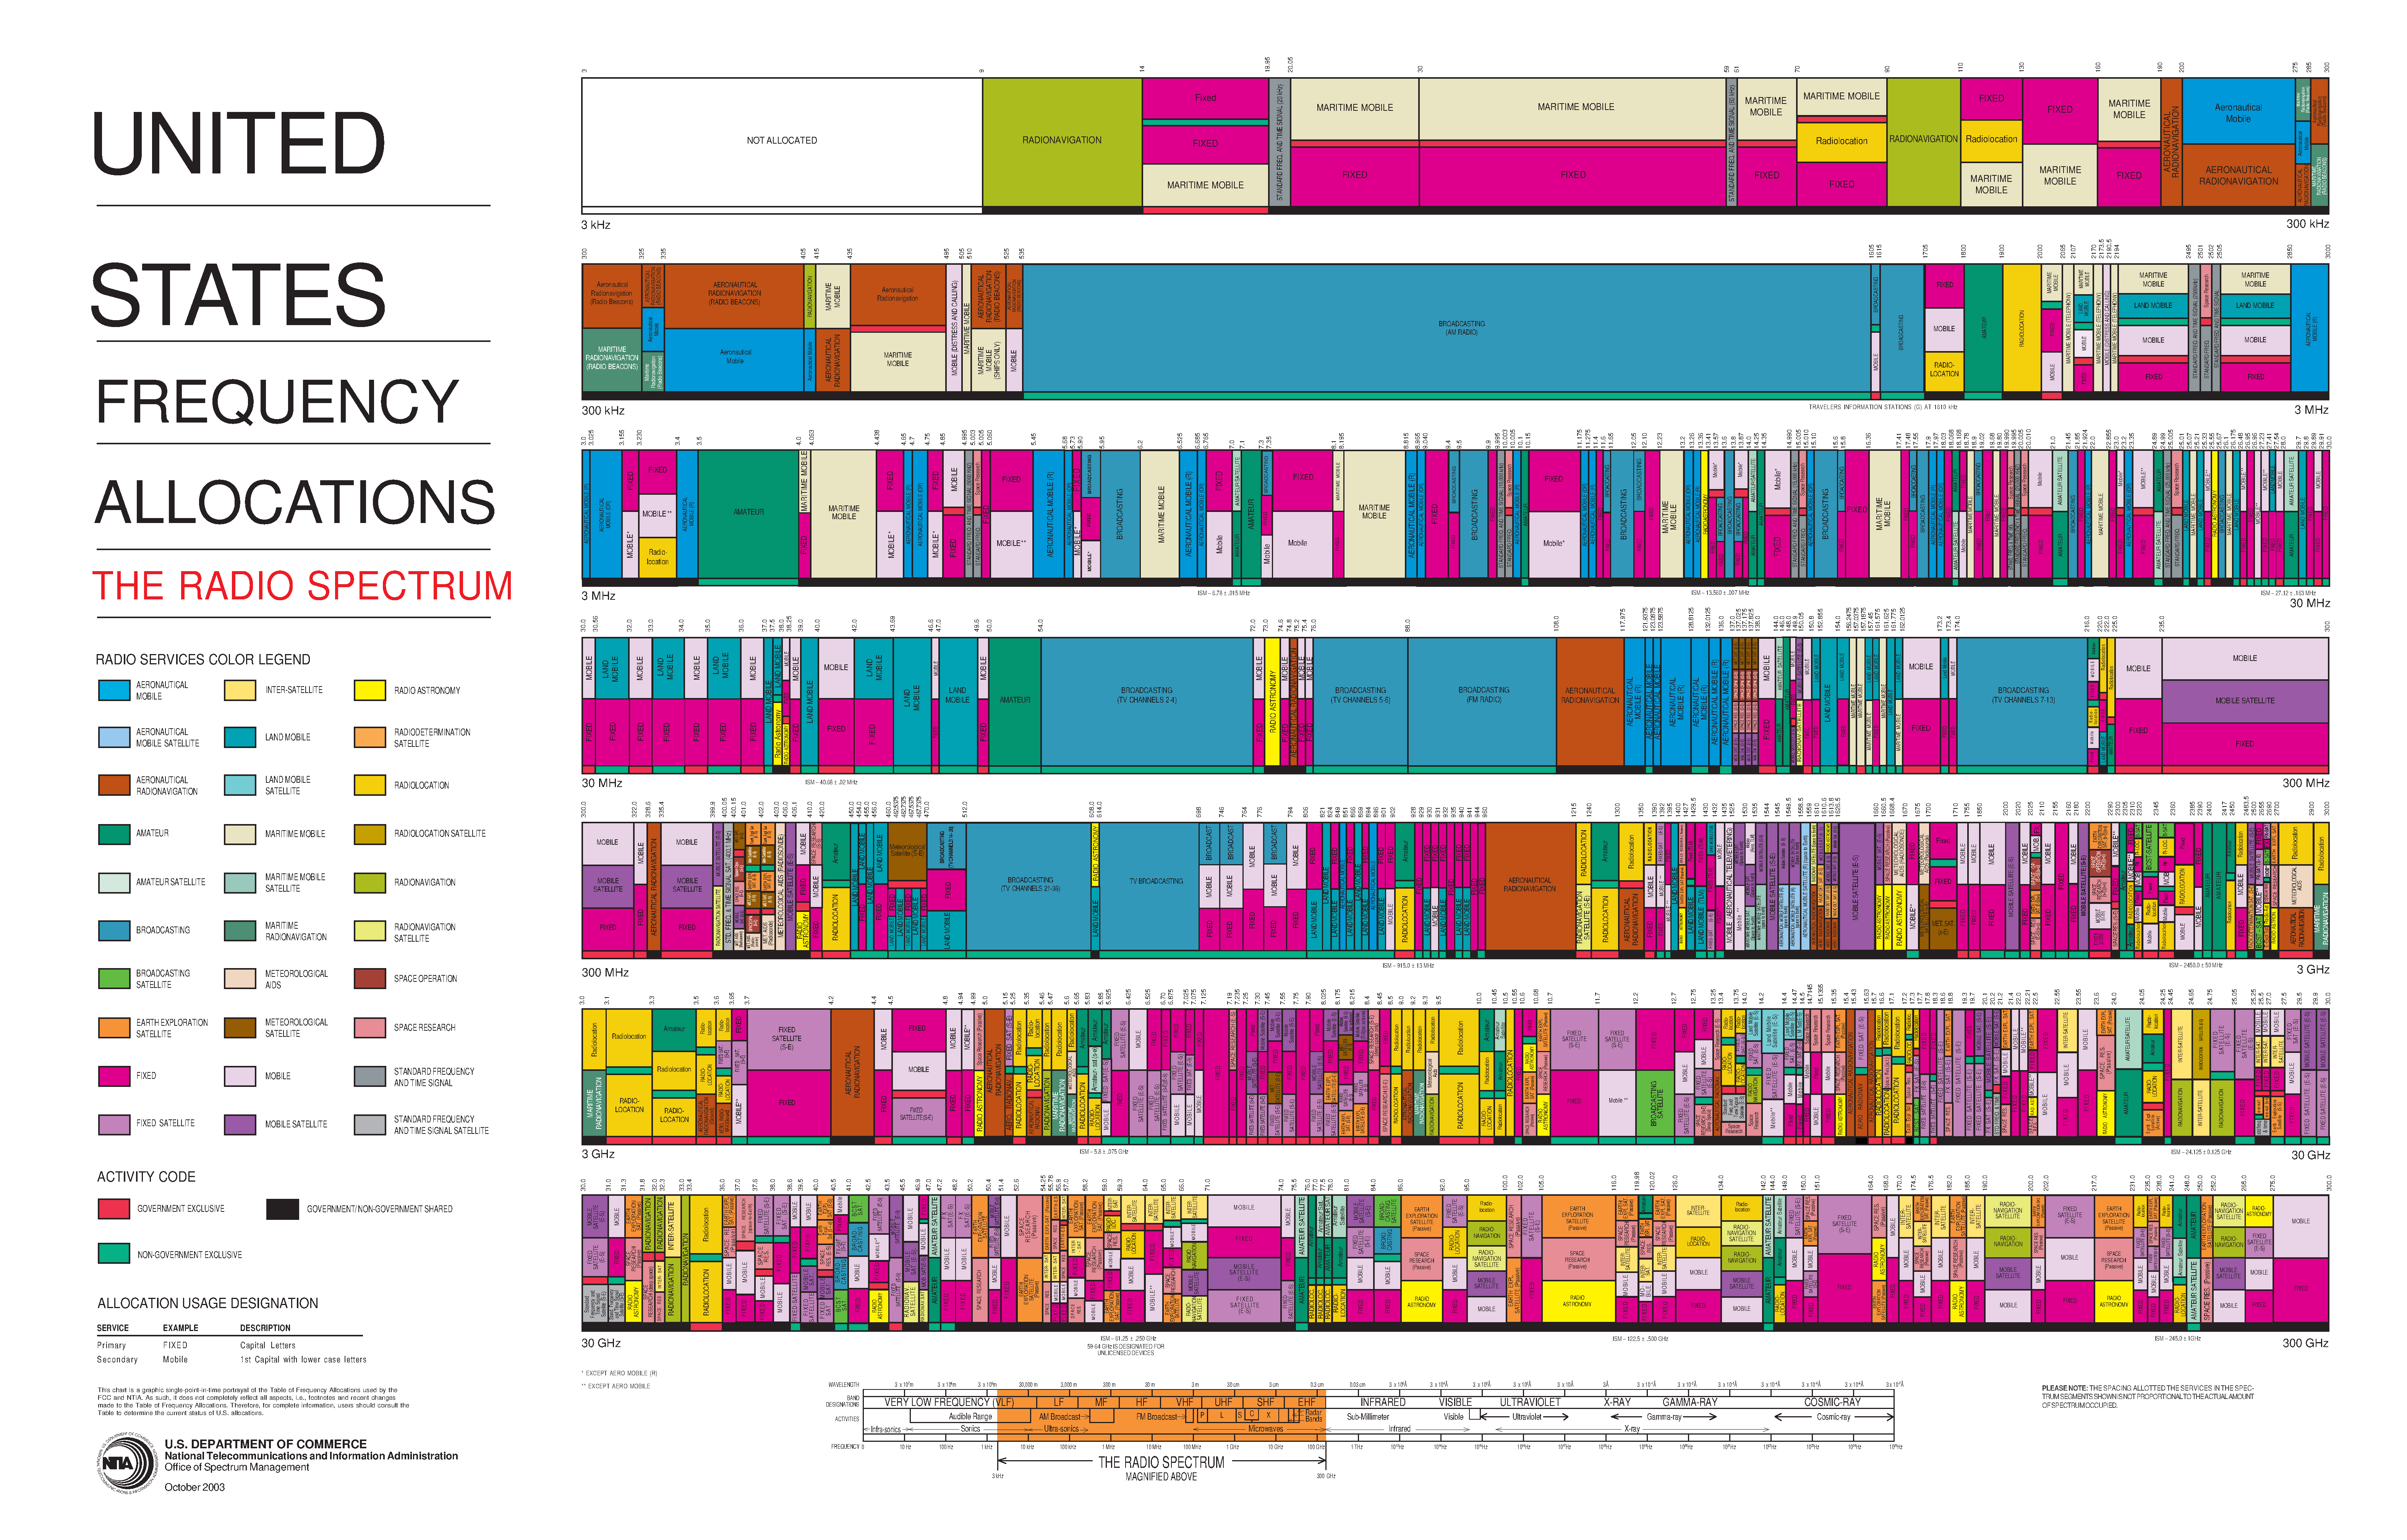
\includegraphics[width=\textwidth, trim={36.5cm 3.1cm 40cm 61cm},clip]{2003-allochrt.pdf}	
		\end{center}
		\legend{Fonte: U.S. Frequency Allocation Chart}
	\end{figure}
	
	Haas (2011) demonstrou factível a realização de transferência de dados utilizando o espectro da luz. Essa comunicação foi chamada de VLC (Visible Light Communication) e posteriormente, como o uso de LED's, de Li-Fi (Light Fidelity) \cite{what-is-lifi}. \par 
	
	Li-Fi possui várias vantagens sobre o comunicações em ondas de rádio que justificam o seu uso \cite{comparison-wifi}. Não há, por exemplo, interferência com as bandas convencionais (como 2.4GHz e 5GHz), sendo portanto compatível com infraestruturas híbridas. Com a largura de banda 10000 vezes maior do que a de RFC, é possível hospedar uma quantidade muito maior de clientes. Nota-se também a alta eficiência do Li-Fi, pois o LED utilizado para transmissão consome pouca energia. Pode-se citar o diferencial de que a luz não atravessa paredes, garantindo segurança e privacidade à rede. Por fim, essa tecnologia tem baixo custo de implementação relativo, uma vez que requer menos componentes do que o Wi-Fi, tornando-a mais barata. \par
	
	Tendo analisado as vantagens, o trabalho a ser realizado visa desenvolver um produto que se utiliza da comunicação Li-Fi para realizar troca de dados entre dispositivos. Produtos que usam essa tecnologia ainda não são fabricados no nível comercial em grande escala, portanto é relevante estudar neste projeto maneiras de viabilizar seu desenvolvimento para uso em pequenos ambientes internos. Seguindo a norma 802.15.7 \cite{lifi-standard}, o grupo tem o intuito de criar um transmissor em formato de luminária e um receptor portátil anexado ao telefone celular. A comunicação deve ser full-duplex entre os dois módulos criados, para que o telefone realize requisições de mídia e a luminária forneça conteúdo para o telefone. Como não existe tal funcionalidade nativa no celular, deve-se criar um aplicativo para Android que realize tradução Li-Fi para dados de mídia. Posteriormente, pode-se integrar o módulo da lamparina à internet ou a redes externas.

	
	\section{Motivação}\label{sec-motivacao}
	
	Este projeto tem como antecedentes experiências com comunicação via luz visível. Criadas no contexto de uma disciplina de laboratório de processadores, as principais motivações foram a maior eficiência energética da VLC, bem como a diminuição de interferência com ondas de radiofrequência. No entanto, estas experiências esbarraram em desafios, principalmente relacionados à falta de um padrão de comunicação e de componentes adequados. Além disso, houve problemas relacionados à capacidade de processamento do microcontrolador utilizado, o que é consequência de um levantamento de requisitos incompleto.
	
	Sendo assim, este projeto surge como um amadurecimento dos objetivos anteriores. Neste segundo momento, foi escolhida uma norma que atendesse às expectativas de implementar comunicação por luz visível de forma eficiente. O padrão IEEE 802.15.7 apresenta a vantagem de ter se completado em dezembro de 2011 e já ter se consolidado entre companhias e grupos industriais que formam o Consórcio Li-Fi. Além disso, o rigor metodológico é uma das preocupações centrais do novo trabalho, o que inclui um refinamento na maneira de definir os requisitos do sistema.
	
	